%!TEX root = ../../report.tex

\subsubsection{Cellular Automaton} % (fold)
\label{ssub:cellular_automaton}

It's a model of a system of cells within a grid with a determined shape, each of this cells can be on one of a finite set of states. It evolves during a finite amount of time steps with a set of simple rules according with the state of the neighbouring cells.
The neighbourhood of the cell can be defined in many different ways, the most common is the use of the adjacent cells. 

In the case where each cell have two possible states and the next generation state depends only on the previous state of the cell and the two immediate neighbors is called an \emph{elementary cellular automaton}. In this case we have $2^3 = 8$ possible patterns for a neighborhood and $2^8 = 256$ sets of possible different rules. This rules are reffered by their \emph{Wolfram code}, defined by Wolfram. 

A common initial state for yhis elementary cellular automata is a random line. But to able to compare the results between rules and get clean results other option is to start with a line with zeros except the middle cell with one. Applying this second option and the following set of rules (the rule 30):

\begin{figure}[htbp]
	\centering
	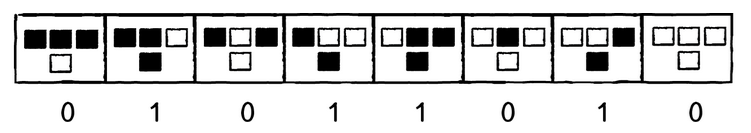
\includegraphics[width=0.85\textwidth]{img/Theory/Cellular_A/Rules.png}
	\caption{Example Production Rules\cite{Shiffman2012}}
	\label{fig:label}
\end{figure}

we get the pattern in the Figure~\ref{fig:resultCA} that represents the evolution of this Cellular automaton over generations:

\begin{figure}[H]
    \centering
    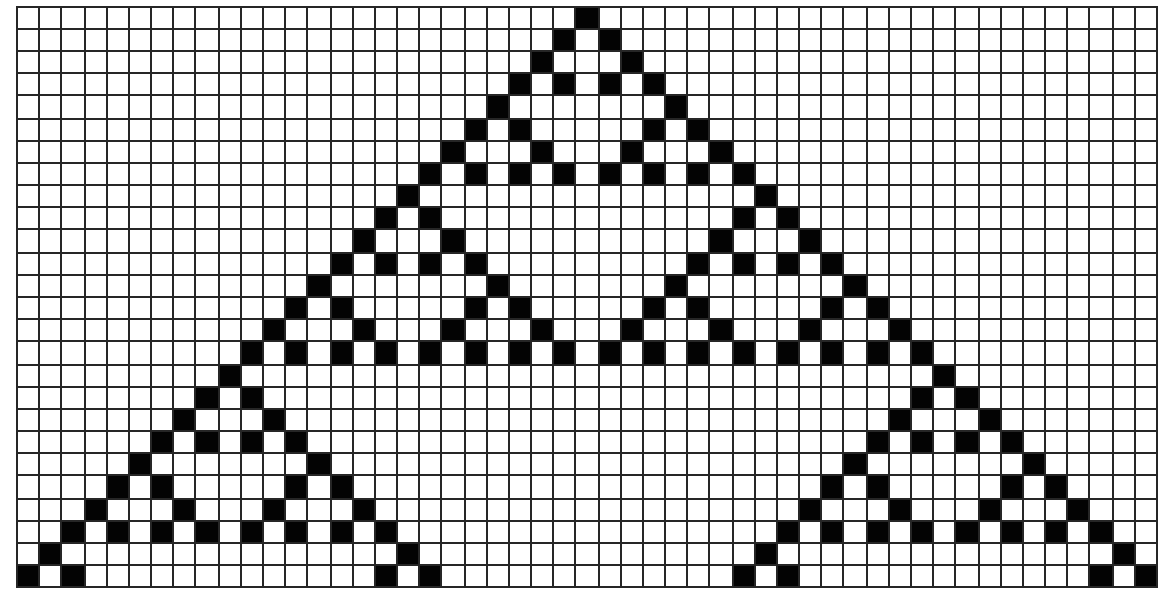
\includegraphics[width=0.75\textwidth]{img/Theory/Cellular_A/Result.png}
    \caption{Sierpiński Triangle, rule 90}
    \label{fig:resultCA}
\end{figure}


In Figure~\ref{fig:resultCA} each line represents an iteration of the system with the application of the rules. With this set of rules a Sierpiński triangle is reproduced.


Cellular automata are used mainly to model phenomena that occurs in the physical world, most of them can only express the basic idea of a phenomenon but some are accurate enough to be able to make predictions.

In this context, cellular automata are used to model natural shapes and textures, the Figure~\ref{fig:CAshell} shows a natural texture on a Textile Cone Snail that looks like the patterns formed with the cellular automaton in the Figure~\ref{fig:CArule30}.



\begin{figure}
        \centering
        \begin{subfigure}[b]{0.6\textwidth}
                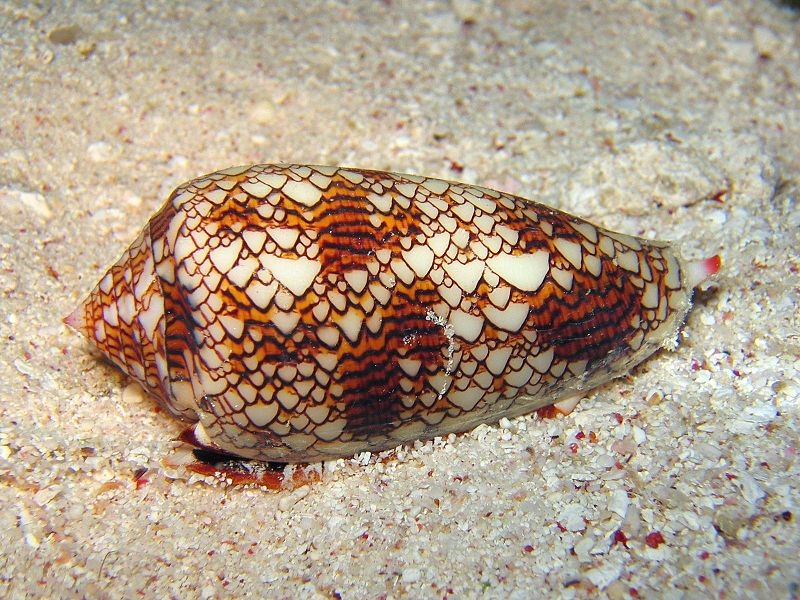
\includegraphics[width=\textwidth]{img/Theory/Cellular_A/shell.jpeg}
                \caption{a)}
				\label{fig:CAshell}
        \end{subfigure}%
        %~ %add desired spacing between images, e. g. ~, \quad, \qquad, \hfill etc.
          %(or a blank line to force the subfigure onto a new line)

        \begin{subfigure}[b]{0.9\textwidth}
                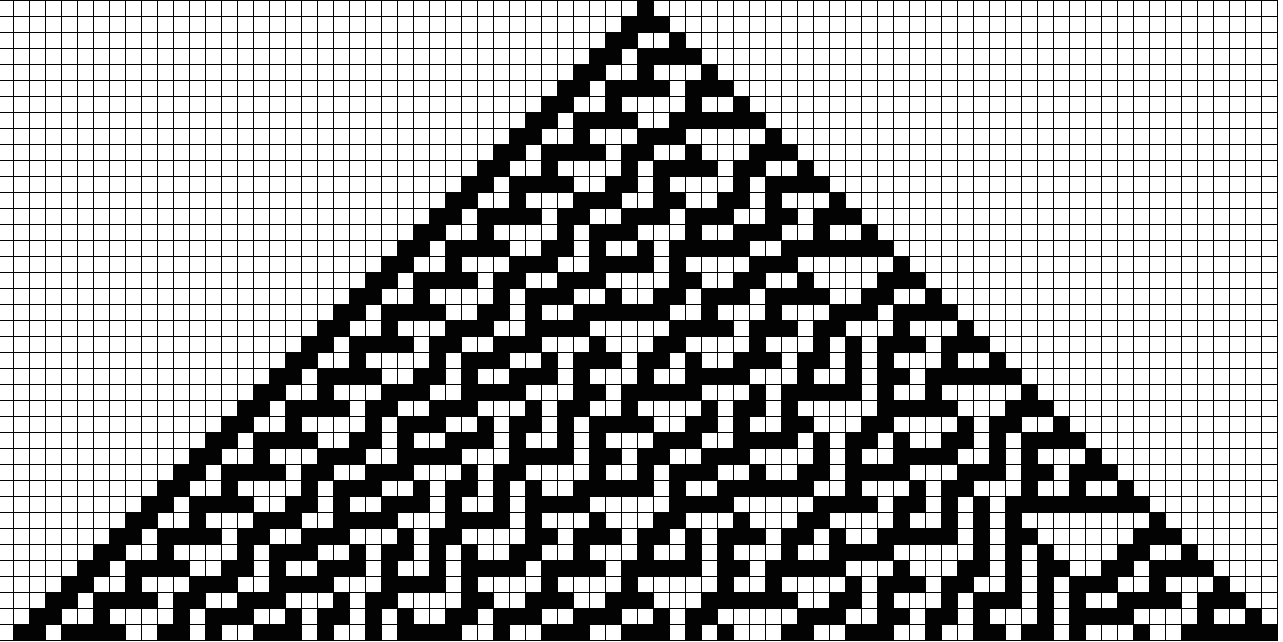
\includegraphics[width=\textwidth]{img/Theory/Cellular_A/Rule30.png}
				\caption{b)}
				\label{fig:CArule30}
        \end{subfigure}
        \caption{Example of the representation of natural patterns with cellular automata. a) Natural Shell, image from \cite{Shiffman2012}. b) Pattern formed with the rule 30.}
		\label{fig:CArule30shell}
\end{figure}



% subsubsection cellular_automaton (end)